%% file: template.tex = LaTeX template for article-like report 
%% init: sometime 1993
%% last: Oct  2 2016  Rob Rutten  Deil
%% site: http://www.staff.science.uu.nl/~rutte101/rrweb/rjr-edu/manuals/student-report/

%% First read ``latex-bibtex-simple-manual.txt'' at
%% http://www.staff.science.uu.nl/~rutte101/Report_recipe.html

%% Start your report production by copying this file into your XXXX.tex.
%% Small changes to the header part will make it an A&A or ApJ manuscript.

%%%%%%%%%%%%%%%%%%%%%%%%%%%%%%%%%%%%%%%%%%%%%%%%%%%%%%%%%%%%%%%%%%%%%%%%%%%%
\documentclass{aa}   %% Astronomy & Astrophysics style class v8.2

\usepackage{graphicx,natbib,url,twoopt}
\usepackage[varg]{txfonts}           %% A&A font choice
\usepackage{hyperref}                %% for pdflatex
%%\usepackage[breaklinks]{hyperref}  %% for latex+dvips
%%\usepackage{breakurl}              %% for latex+dvips
\usepackage{pdfcomment}              %% for popup acronym meanings
\usepackage{acronym}                 %% for popup acronym meanings

\hypersetup{
  colorlinks=true,   %% links colored instead of frames
  urlcolor=blue,     %% external hyperlinks
  linkcolor=red,     %% internal latex links (eg Fig)
}

\bibpunct{(}{)}{;}{a}{}{,}    %% natbib cite format used by A&A and ApJ

\pagestyle{plain}   %% undo the fancy A&A pagestyle 

%% Add commands to add a note or link to a reference
\makeatletter
\newcommand{\bibnote}[2]{\global\@namedef{#1note}{#2}}
\newcommand{\biblink}[2]{\global\@namedef{#1link}{#2}}
\makeatother

%% Commands to make citations ADS clickers and to add such also to refs
%% May 2014: they give error stops ("Illegal parameter number ..."}
%%   for plain latex with TeX Live 2013; the ad-hoc fixes added below let
%%   latex continue instead of stop within these commands.
%%   Please let me know if you know a better fix!
%%   No such problem when using pdflatex.
\makeatletter
 \newcommandtwoopt{\citeads}[3][][]{%
   \nonstopmode%              %% fix to not stop at error message in latex
   \href{http://adsabs.harvard.edu/abs/#3}%
        {\def\hyper@linkstart##1##2{}%
         \let\hyper@linkend\@empty\citealp[#1][#2]{#3}}%   %% Rutten, 2000
   \biblink{#3}{\href{http://adsabs.harvard.edu/abs/#3}{ADS}}%
   \errorstopmode}            %% fix to resume stopping at error messages 
 \newcommandtwoopt{\citepads}[3][][]{%
   \nonstopmode%              %% fix to not stop at error message in latex
   \href{http://adsabs.harvard.edu/abs/#3}%
        {\def\hyper@linkstart##1##2{}%
         \let\hyper@linkend\@empty\citep[#1][#2]{#3}}%     %% (Rutten 2000)
   \biblink{#3}{\href{http://adsabs.harvard.edu/abs/#3}{ADS}}%
   \errorstopmode}            %% fix to resume stopping at error messages
 \newcommandtwoopt{\citetads}[3][][]{%
   \nonstopmode%              %% fix to not stop at error message in latex
   \href{http://adsabs.harvard.edu/abs/#3}%
        {\def\hyper@linkstart##1##2{}%
         \let\hyper@linkend\@empty\citet[#1][#2]{#3}}%     %% Rutten (2000)
   \biblink{#3}{\href{http://adsabs.harvard.edu/abs/#3}{ADS}}%
   \errorstopmode}            %% fix to resume stopping at error messages 
 \newcommandtwoopt{\citeyearads}[3][][]{%
   \nonstopmode%              %% fix to not stop at error message in latex
   \href{http://adsabs.harvard.edu/abs/#3}%
        {\def\hyper@linkstart##1##2{}%
         \let\hyper@linkend\@empty\citeyear[#1][#2]{#3}}%  %% 2000
   \biblink{#3}{\href{http://adsabs.harvard.edu/abs/#3}{ADS}}%
   \errorstopmode}            %% fix to resume stopping at error messages 
\makeatother

%% ADS specific page opener = {bibcode}{pdf page number}{link text}
\def\linkadspage#1#2#3{\href{http://adsabs.harvard.edu/cgi-bin/nph-data_query?bibcode=#1\&link_type=ARTICLE\&d_key=AST\#page=#2}{#3}}

%% Acronyms
\newacro{ADS}{Astrophysics Data System}
\newacro{NLTE}{non-local thermodynamic equilibrium}
\newacro{NASA}{National Aeronautics and Space Administration}

%% Add popups with meaning to acronyms 
%% NB: only show up in Adobe Reader and do not work with \input or \include
\gdef\acp#1{%
  \pdfmarkupcomment[markup=Underline,color={1 1 1},author={{#1}},opacity=0]%
  {{#1}}{{\acl{#1}}}}

%% Spectral species
\def\MgI{\ion{Mg}{I}}          %% A&A; for aastex use \def\MgI{\ion{Mg}{1}} 
\def\MgII{\ion{Mg}{II}}        %% A&A; for aastex use \def\MgII{\ion{Mg}{2}} 

%% Hyphenation
\hyphenation{Schrij-ver}       %% Dutch ij is a single character

%%%%%%%%%%%%%%%%%%%%%%%%%%%%%%%%%%%%%%%%%%%%%%%%%%%%%%%%%%%%%%%%%%%%%%%%%%%%
\begin{document}  

%% simple header.  Change into A&A or ApJ commands for those journals

\twocolumn[{%
\vspace*{4ex}
\begin{center}
  {\Large \bf Compare the multi-wavelength positions of quasars}\\[4ex]       
  {\large \bf Niu Liu
%              Niu Liu $^{1, 2}$, 
%              S\'ebastien Lambert$^2$,
%              Cheng-Yu Ding $^1$,
%              Zi Zhu $^1$,
%              and 
%              Jia-Cheng Liu $^1$
          }\\[4ex]
  \begin{minipage}[t]{15cm}
%        $^1$ Institute1\\
%        $^2$ Institute2\\
%        $^3$ Institute3\\

  {\bf Abstract.}  I compare the quasar positions measured at four different bands, that is, optical, X-, K-, and Ka-band, 
  in oder to address the radio-to-optical offset.
  

  \vspace*{2ex}
  \end{minipage}
\end{center}
}] 


%%%%%%%%%%%%%%%%%%%%%%%%%%%%%%%%%%%%%%%%%%%%%%%%%%%%%%%%%%%%%%%%%%%%%%%%%%%%
\section{Introduction}     \label{sec:introduction}
%%%%%%%%%%%%%%%%%%%%%%%%%%%%%%%%%%%%%%%%%%%%%%%%%%%%%%%%%%%%%%%%%%%%%%%%%%%%

To be completed later\dots


%% {fig:XX}
%===========================================================================
%\begin{figure}[hbtp]
%  \centering
%  \includegraphics[width=80mm]{XX}
%  \caption[]{\label{fig:XX}
%    Caption text \dots
%  }
%\end{figure}
%===========================================================================


%%%%%%%%%%%%%%%%%%%%%%%%%%%%%%%%%%%%%%%%%%%%%%%%%%%%%%%%%%%%%%%%%%%%%%%%%%%%
\section{Materials}    \label{sec:obs}
%%%%%%%%%%%%%%%%%%%%%%%%%%%%%%%%%%%%%%%%%%%%%%%%%%%%%%%%%%%%%%%%%%%%%%%%%%%%

I used the three components of ICRF3 catalog to provide the quasar positions at S/X-, K-, and X/Ka-band.
For the optical domain, the \texttt{gaiadr2.aux\_iers\_gdr2\_cross\_id} sample from the {\it Gaia} DR2 was used.
A cross-match amongst these four catalogs gave a list of 488 common objects.
Using the S/X position as the reference position, I calculated the position offsets for other three bands.
The position angle (PA) of the position offsets was determined to indicate the direction of position offset.
As illustrated in Fig.~\ref{fig:illustration-diagram}, the PA is counted from the positive increasing of the declination to the increasing direction of the right ascension.


%% {fig:illustration-diagram}
%===========================================================================
\begin{figure}[hbtp]
  \centering
  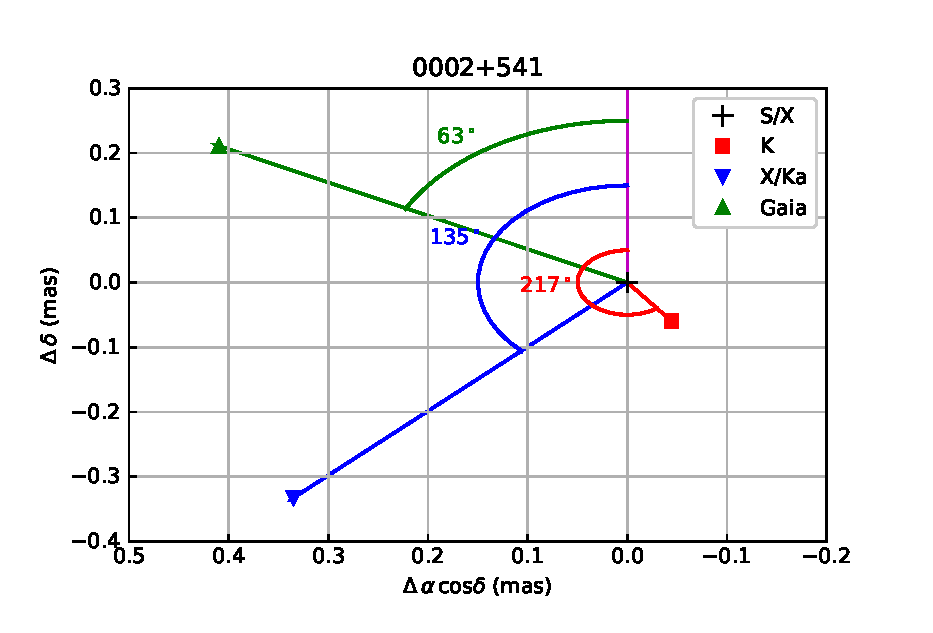
\includegraphics[width=80mm]{figs/illustration-diagram}
  \caption[]{\label{fig:illustration-diagram}
    Position offset and its position angle for quasar `0002+541'.
    The increasing direction of right ascension points towards the left, which is consistent to the convention of VLBI imaging.
  }
\end{figure}
%===========================================================================


%%%%%%%%%%%%%%%%%%%%%%%%%%%%%%%%%%%%%%%%%%%%%%%%%%%%%%%%%%%%%%%%%%%%%%%%%%%%
\section{Analaysis}    \label{sec:analysis}
%%%%%%%%%%%%%%%%%%%%%%%%%%%%%%%%%%%%%%%%%%%%%%%%%%%%%%%%%%%%%%%%%%%%%%%%%%%%

%%%%%%%%%%%%%%%%%%%%%%%%%%%%%%%%%%%%%%%%%%%%%%%%%%%%%%%%%%%%%%%%%%%%%%%%%%%%
\subsection{Systematics}    \label{subsec:systematics}
%%%%%%%%%%%%%%%%%%%%%%%%%%%%%%%%%%%%%%%%%%%%%%%%%%%%%%%%%%%%%%%%%%%%%%%%%%%%
I first looked at the position offset as a function of the right ascension and declination.
This step is intended to check the possible systematics between different celestial reference frames.
Figures~\ref{fig:k-sx-pos-offset}-\ref{fig:gdr2-sx-pos-offset} display the offset of K-band, X/Ka-band, and Gaia (optical) positions with respect to the S/X-band position as functions of right ascension and declination.
For `K$-$S/X', the position offset together with its quoted formal uncertainty (indicated by the error bar) increases from the north to the south.
This holds true also for `X/Ka$-$S/X' but not for `Gaia$-$S/X'.
It is easy to understand since the VLBI position has an asymmetry in the south-north direction, that is, the measured position formal error of quasars in the south is generally worse that those in the north.
Another feather for `K$-$S/X' is that offset in the right ascension (at the level of 0.1\,mas) is smaller than in the declination (at the level of 0.3\,mas). 
The `X/Ka$-$S/X' offset show an obvious dependency on the declination and a declination bias in the south, as indicated in the right panel of Fig.~\ref{fig:xka-sx-pos-offset}.
This will surely bias the calculation of position angle for position offset.

Figure~\ref{fig:pa} show the distribution of position angle calculated from position offsets of `K$-$S/X', `X/Ka$-$S/X', and `Gaia$-$S/X'.
One can find the PA for `X/Ka$-$S/X' concentrates in the range of $(150,210)~^\circ$, which is not seen in the case of `K$-$S/X' and `Gaia$-$S/X'.
It is most likely be caused by the systematics presented in Fig.~\ref{fig:xka-sx-pos-offset}.
So it is necessary to remove the global difference and align the other CRF to the S/X-band frame before we address the position angle of position offset.

To align the frame, I use the 16-parameter transformation, that is, the first two orders of VSH functions. 
The sample could be the whole sample of 488 sources, or all the common objects between each two-pair catalogs.
Here I used the later and no more selection was done to the sample for getting a `clean' sample.
Tables~\ref{table:vsh01}-\ref{table:vsh01} gives the transformation parameters from  a least square fitting.

%% {fig:k-sx-pos-offset}
%===========================================================================
\begin{figure*}[hbtp]
    \centering
    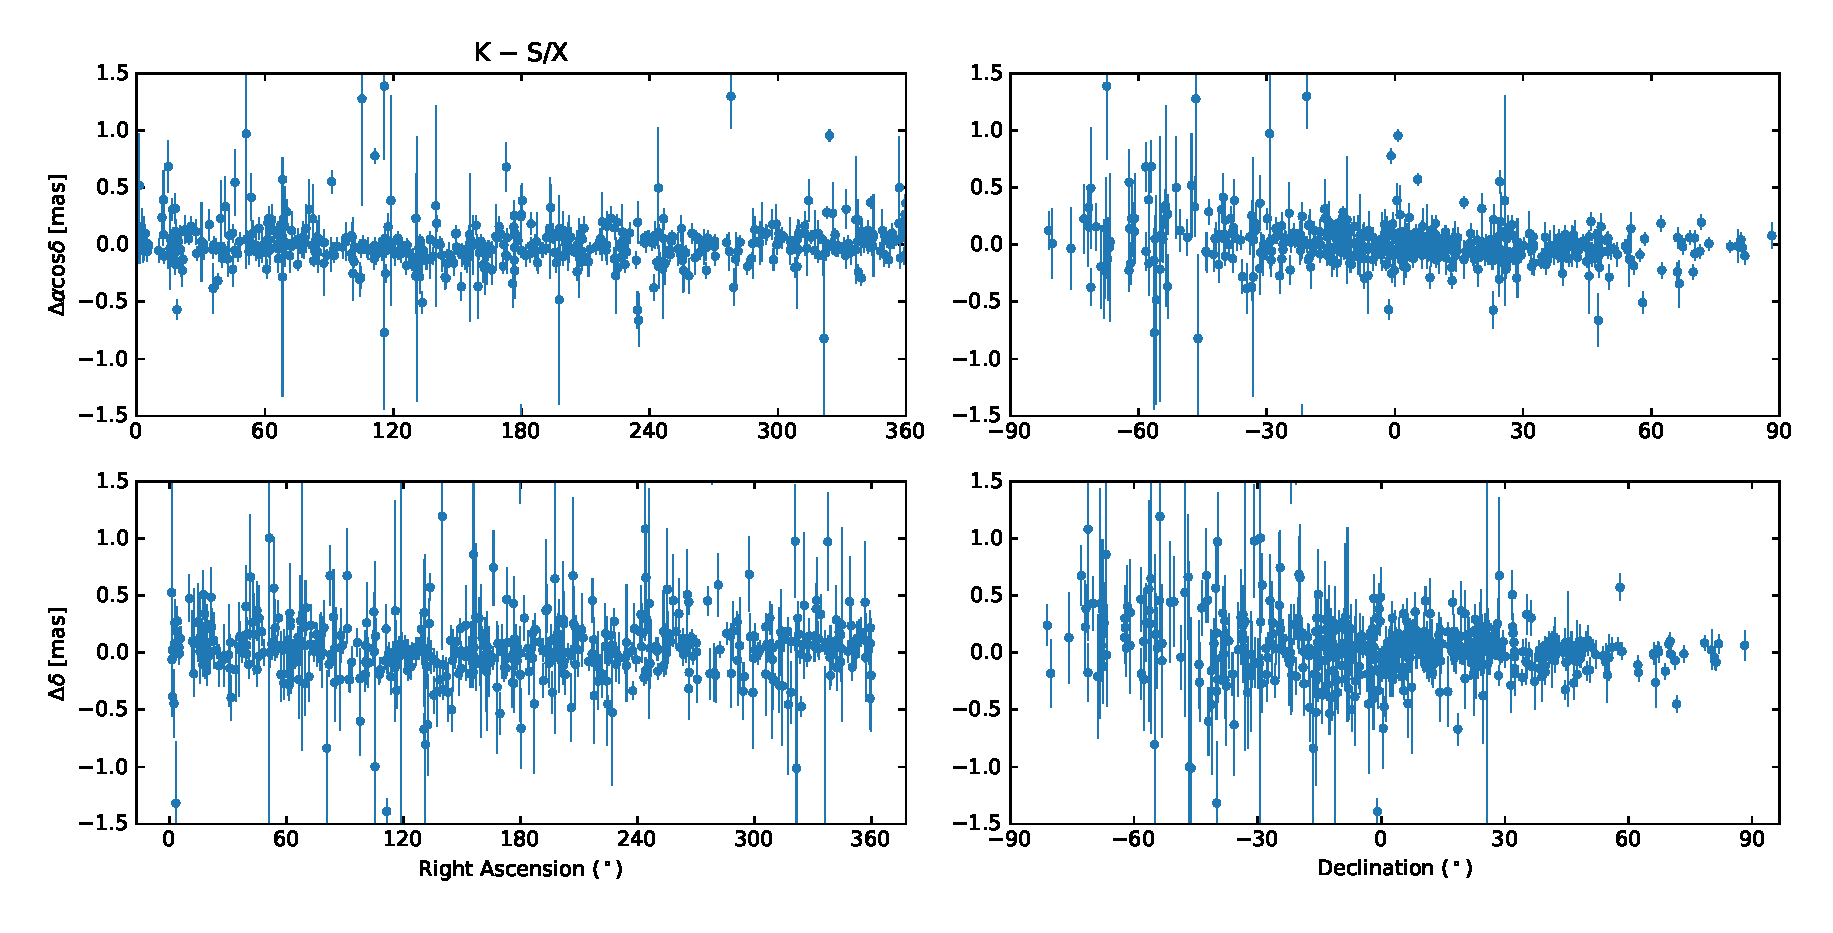
\includegraphics[width=160mm]{figs/k-sx-pos-offset}
    \caption[]{\label{fig:k-sx-pos-offset}
        Position offset for common objects between S/X and K, in the sense of `K$-$S/X'.
        The limit of the position offset is set as 1.5\,mas in oder to show the dependency on the right ascension and declination.
        As a result, several objects are beyond the plots.
    }
\end{figure*}
%===========================================================================

%% {fig:xka-sx-pos-offset}
%===========================================================================
\begin{figure*}[hbtp]
    \centering
    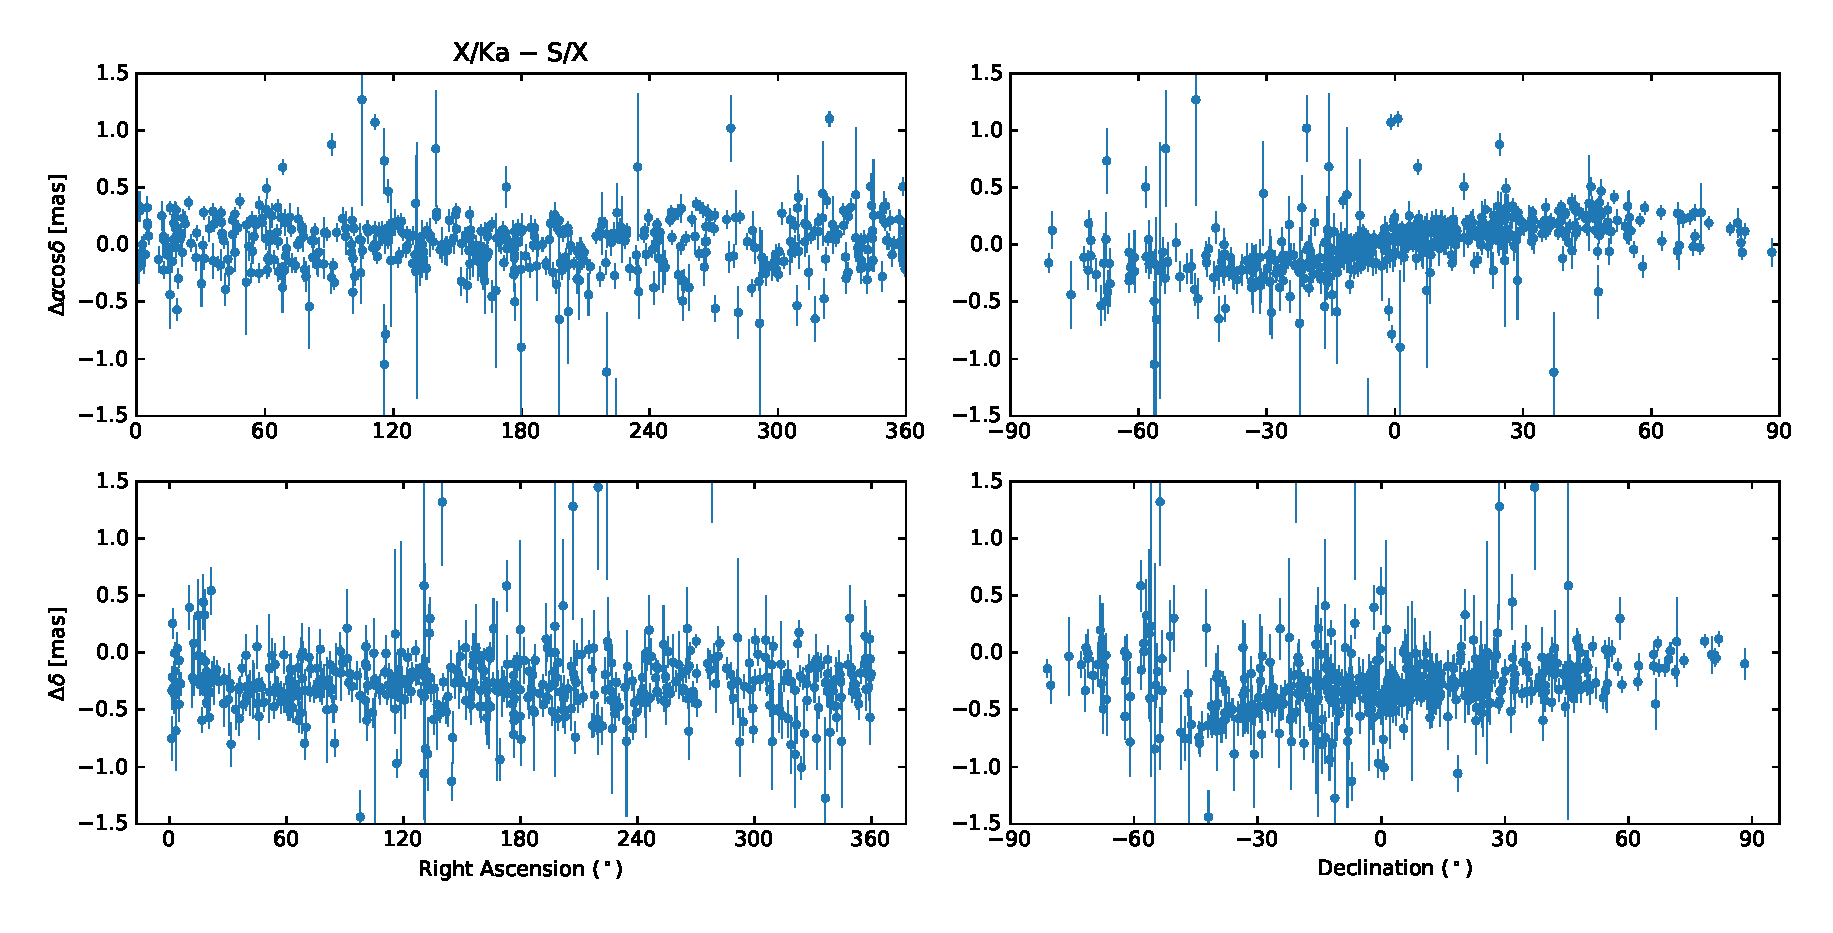
\includegraphics[width=160mm]{figs/xka-sx-pos-offset}
    \caption[]{\label{fig:xka-sx-pos-offset}
        Position offset for common objects between S/X and X/Ka, in the sense of `X/Ka$-$S/X'.
        The limit of the position offset is set as 1.5\,mas in oder to show the dependency on the right ascension and declination.
        As a result, several objects are beyond the plots.
    }
\end{figure*}
%===========================================================================

%% {fig:gdr2-sx-pos-offset}
%===========================================================================
\begin{figure*}[hbtp]
    \centering
    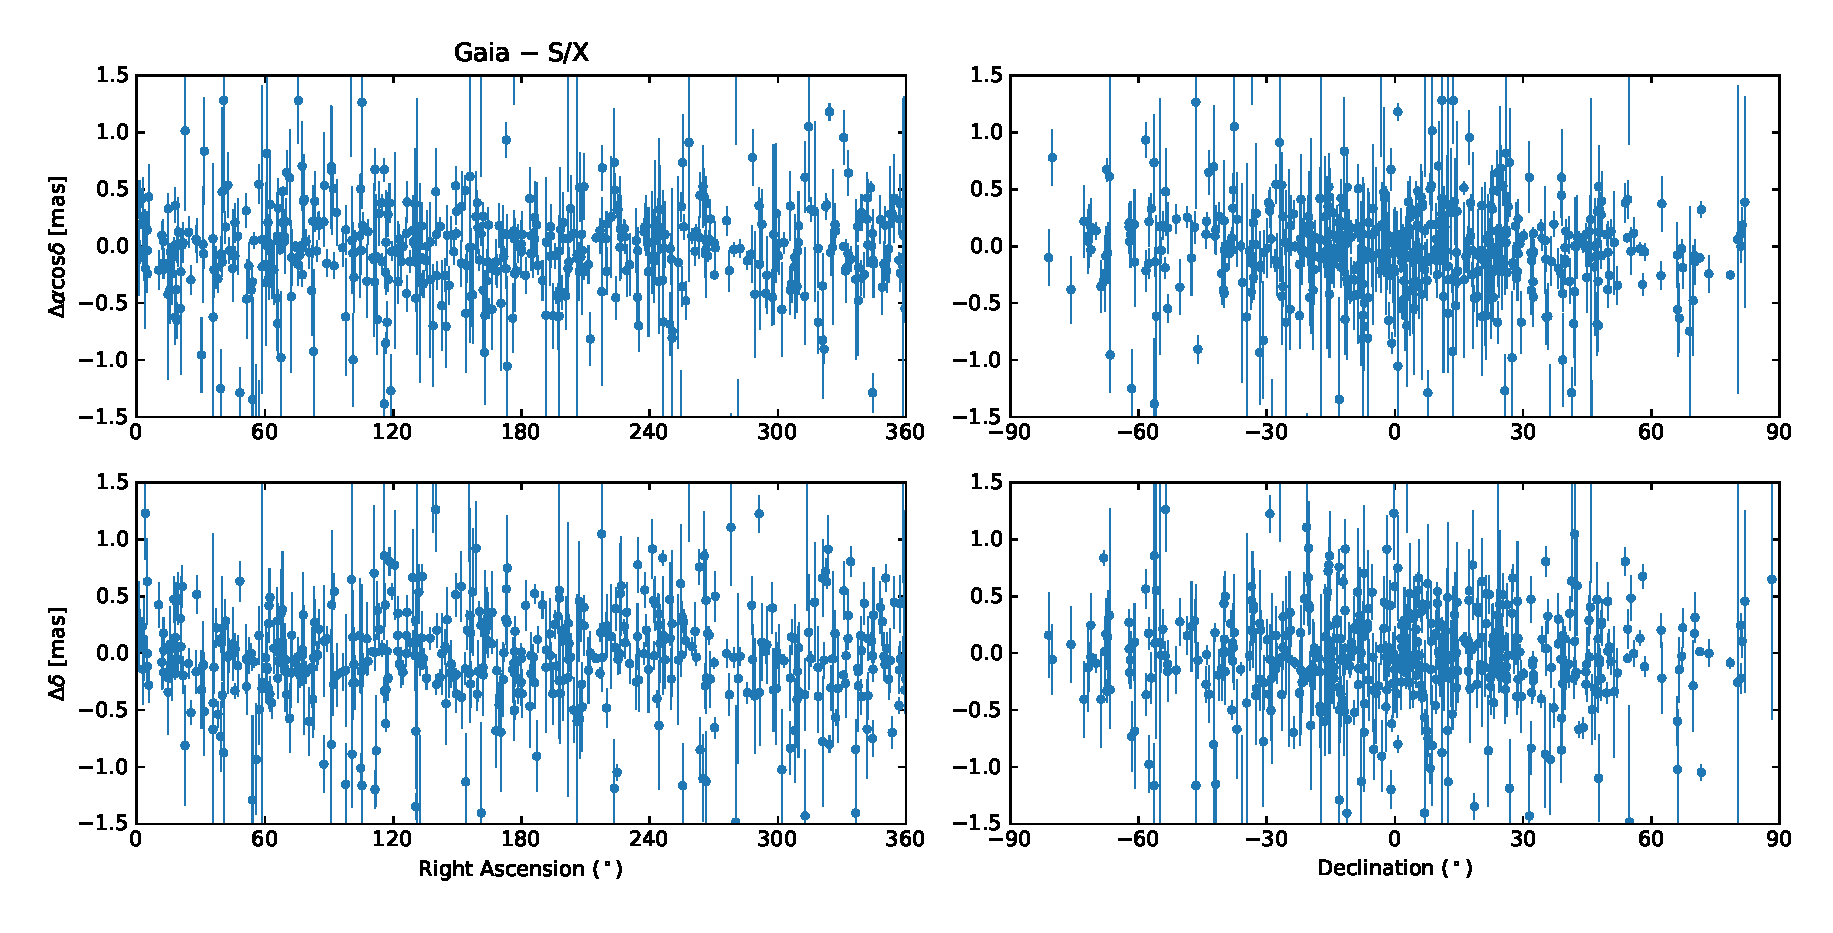
\includegraphics[width=160mm]{figs/gdr2-sx-pos-offset}
    \caption[]{\label{fig:gdr2-sx-pos-offset}
        Position offset for common objects between S/X and Gaia, in the sense of `Gaia$-$S/X'.
        The limit of the position offset is set as 1.5\,mas in oder to show the dependency on the right ascension and declination.
        As a result, several objects are beyond the plots.
    }
\end{figure*}
%===========================================================================

%% {fig:pa}
%===========================================================================
\begin{figure}[hbtp]
    \centering
    \includegraphics[width=80mm]{figs/pa-hist}
    \caption[]{\label{fig:pa}
        Distribution of the position angle of position offset for `K$-$S/X', `X/Ka$-$S/X', and `Gaia$-$S/X'.
    }
\end{figure}
%===========================================================================

%% {tanle:table:vsh01}
%===========================================================================
\begin{table*}[htbp]
	\center
    \caption{\label{table:vsh01}
        Orientation and glide of ICRF3 K, X/Ka, and Gaia DR2 w.r.t. ICRF3 S/X. 
        Unit: $\mathrm{\mu as}$.}
    \begin{tabular}{cccccccc}
        \hline \hline
        Catalog  &Sources & $R_1$ & $R_2$ & $R_3$ & $D_1$ & $D_2$ & $D_3$ \\[0.1cm]
        \hline 
        ICRF3 K    & 793 &$ -15\pm  30$  &$-17 \pm  29$ &$+ 8 \pm  15$ &$-17 \pm  25$ &$+51 \pm  26$ &$+26 \pm  28$ \\
        ICRF3 X/Ka & 638 &$ -27\pm  11$  &$- 2 \pm  11$ &$+17 \pm   7$ &$+ 7 \pm  10$ &$+35 \pm  10$ &$-354\pm  11$ \\
        Gaia DR2   &2820 &$ +32 \pm 33$  &$-47 \pm  31$ &$-44 \pm  30$ &$-28 \pm  32$ &$+49 \pm  31$ &$-14 \pm  32$ \\
        \hline
    \end{tabular}
\end{table*}
%===========================================================================

%% {tanle:table:vsh02}
%===========================================================================
\begin{table*}[htbp]
	\center
    \caption{\label{table:vsh02}
        Quadrupolar terms of ICRF3 K, X/Ka, and Gaia DR2 w.r.t. ICRF3 S/X. 
        Unit: $\mathrm{\mu as}$.}
    \begin{tabular}{ccccccccccc}
        \hline \hline
Catalogs    &$E_{22}^R$  &$E_{22}^I$  &$E_{21}^R$  &$E_{21}^I$  &$E_{20}$    &$M_{22}^R$  &$M_{22}^I$  &$M_{21}^R$  &$M_{21}^I$  &$M_{20}$    \\ [0.1cm]
\hline
ICRF3 K     &$   -2 \pm    10 $  &$   -3 \pm    10 $  &$  -34 \pm    29 $  &$  -71 \pm    30 $  &$   +7 \pm    33 $  &$   +2 \pm    15 $  &$  -11 \pm    15 $  &$  +15 \pm    30 $  &$  -32 \pm    30 $  &$  -26 \pm    20 $ \\
ICRF3 X/Ka  &$   -3 \pm     5 $  &$    5 \pm     5 $  &$  -33 \pm    12 $  &$   28 \pm    13 $  &$   86 \pm    13 $  &$   -1 \pm     6 $  &$  +10 \pm     6 $  &$   -7 \pm    11 $  &$   -2 \pm    12 $  &$  224 \pm    10 $ \\
Gaia DR2    &$  +37 \pm    19 $  &$   -3 \pm    19 $  &$  +9 \pm    37 $   &$  -50 \pm    40 $  &$  +41 \pm    36 $  &$   +2 \pm    20 $  &$   +1 \pm    20 $  &$  +26 \pm    38 $  &$  +72 \pm    39 $  &$  -12 \pm    33 $ \\
        \hline\end{tabular}
\end{table*}



%%%%%%%%%%%%%%%%%%%%%%%%%%%%%%%%%%%%%%%%%%%%%%%%%%%%%%%%%%%%%%%%%%%%%%%%%%%%
\subsection{Position angle}    \label{subsec:pa}
%%%%%%%%%%%%%%%%%%%%%%%%%%%%%%%%%%%%%%%%%%%%%%%%%%%%%%%%%%%%%%%%%%%%%%%%%%%%
I adjusted the transformation parameters given in Tables~\ref{table:vsh01}-\ref{table:vsh02} to the position offset and recalculate the position angle. 
From now on, all the presented results are based on the adjusted position offset.
The normalized position offset was also calculated to check the result of frame alignments.
Figures~\ref{fig:nor-ra-dec-k-sx-hist}-\ref{fig:nor-ra-dec-gdr2-sx-hist} report these quantities, from which we can find that the declination bias between S/X and X/Ka was removed and the shape of normalized position offset is more close to the Gaussian distribution.
Figure~\ref{fig:rho-x-scatter-nosys} show the normalized separation and angular separation.
If we set a limit of 1\,mas on the angular separation and of $X_0=3.52$ as indicated by the horizontal and vertical line, respectively, just a few tens of sources fell into the upper right corner, even for Gaia and ICRF3 S/X.
It means that most of common objects do not yield a statistically significant position offset for measurements from different frequencies.
This result would possibly bring us some problems in interpretation of position angle.

Figures~\ref{fig:k-sx-scatter-nosys}-\ref{fig:gdr2-sx-scatter-nosyst} demonstrate the scatter of K-band, X/Ka-band, and Gaia position offset with referred to the S/X-band position, respectively.
From these diagrams, we find that the position offsets of K- and X/Ka-band look like a ellipse nearly along the declination, while for Gaia the distribution has a circle-like shape.
If we look at the distribution of these position angle for K-, X/Ka-band, and Gaia position referring to the S/X position (Fig.~\ref{fig:pa-nosys}), we can find a peak at around $0\,^\circ$, $180\,^\circ$, and $360\,^\circ$.
Possibly, the peak is caused by the declination errors in the VLBI catalogs.
Figure~\ref{fig:pa-diff-from-sys} shows the distribution of position angle before and after aligning the frames.
The X/Ka-band shows the largest discrepancy, underlying that the systematics will bias the calculation of position angle.

We want to see the relative position at four bands for an individual quasar.
As a result, I calculated the included angle between the K and X/Ka, K and Gaia, and X/Ka and Gaia.
Figure~\ref{fig:pa-diff-nosys} depicts the distribution of the included angles, where a peak around $0^\circ$ is clearly seen while no peak appears at $180^\circ$.
It indicates that as seen from S/X position of these quasars, the K, X/Ka, and Gaia positions align in the same directions.
And it would be nice if this direction is in the opposite of the jet direction.
  
%% {fig:nor-ra-dec-k-sx-hist}
%===========================================================================
\begin{figure*}[hbtp]
    \centering
    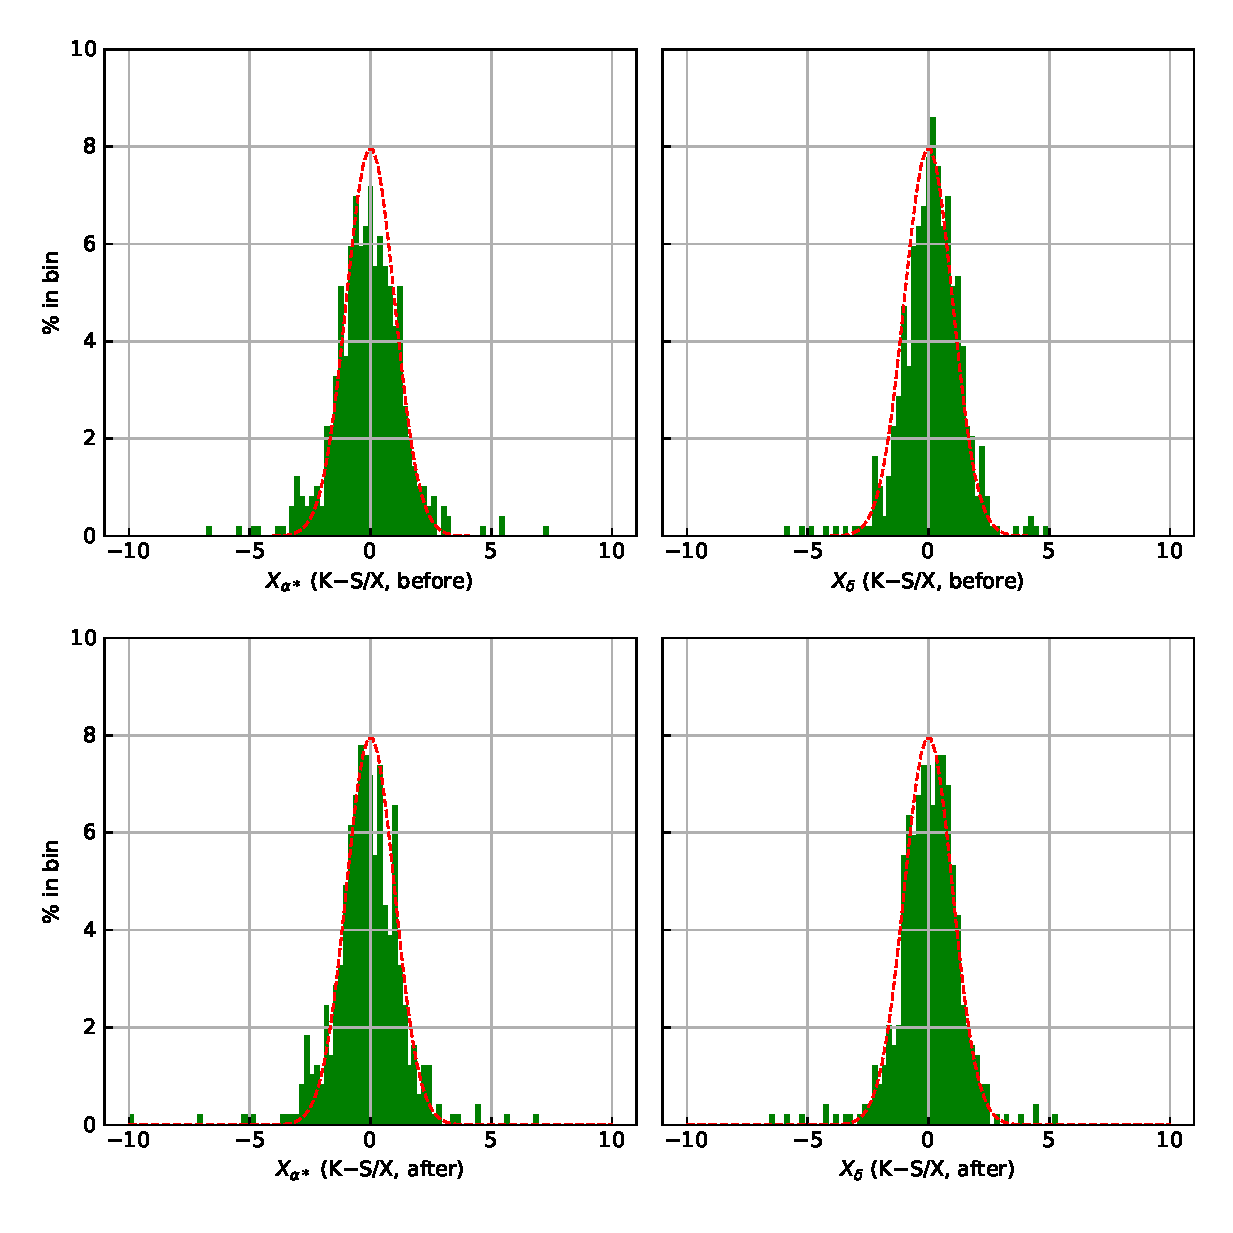
\includegraphics[width=160mm]{figs/nor-ra-dec-k-sx-hist}
    \caption[]{\label{fig:nor-ra-dec-k-sx-hist}
        Normalized position offset for common objects between S/X and K, in the sense of `K$-$S/X' before and after aligning the frame.
        The red dashed line indicates the shape of a Gaussian distribution.
    }
\end{figure*}
%===========================================================================

%% {fig:nor-ra-dec-xka-sx-hist}
%===========================================================================
\begin{figure*}[hbtp]
    \centering
    \includegraphics[width=160mm]{figs/nor-ra-dec-xka-sx-hist}
    \caption[]{\label{fig:nor-ra-dec-xka-sx-hist}
        Normalized position offset for common objects between S/X and X/Ka, in the sense of `X/Ka$-$S/X' before and after aligning the frame.
        The red dashed line indicates the shape of a Gaussian distribution.
    }
\end{figure*}
%===========================================================================

%% {fig:nor-ra-dec-gdr2-sx-hist}
%===========================================================================
\begin{figure*}[hbtp]
    \centering
    \includegraphics[width=160mm]{figs/nor-ra-dec-gdr2-sx-hist}
    \caption[]{\label{fig:nor-ra-dec-gdr2-sx-hist}
        Normalized position offset for common objects between S/X and Gaia, in the sense of `Gaia$-$S/X' before and after aligning the frame.
        The red dashed line indicates the shape of a Gaussian distribution.
    }
\end{figure*}
%===========================================================================

%% {fig:rho-x-scatter-nosys}
%===========================================================================
\begin{figure}[hbtp]
    \centering
    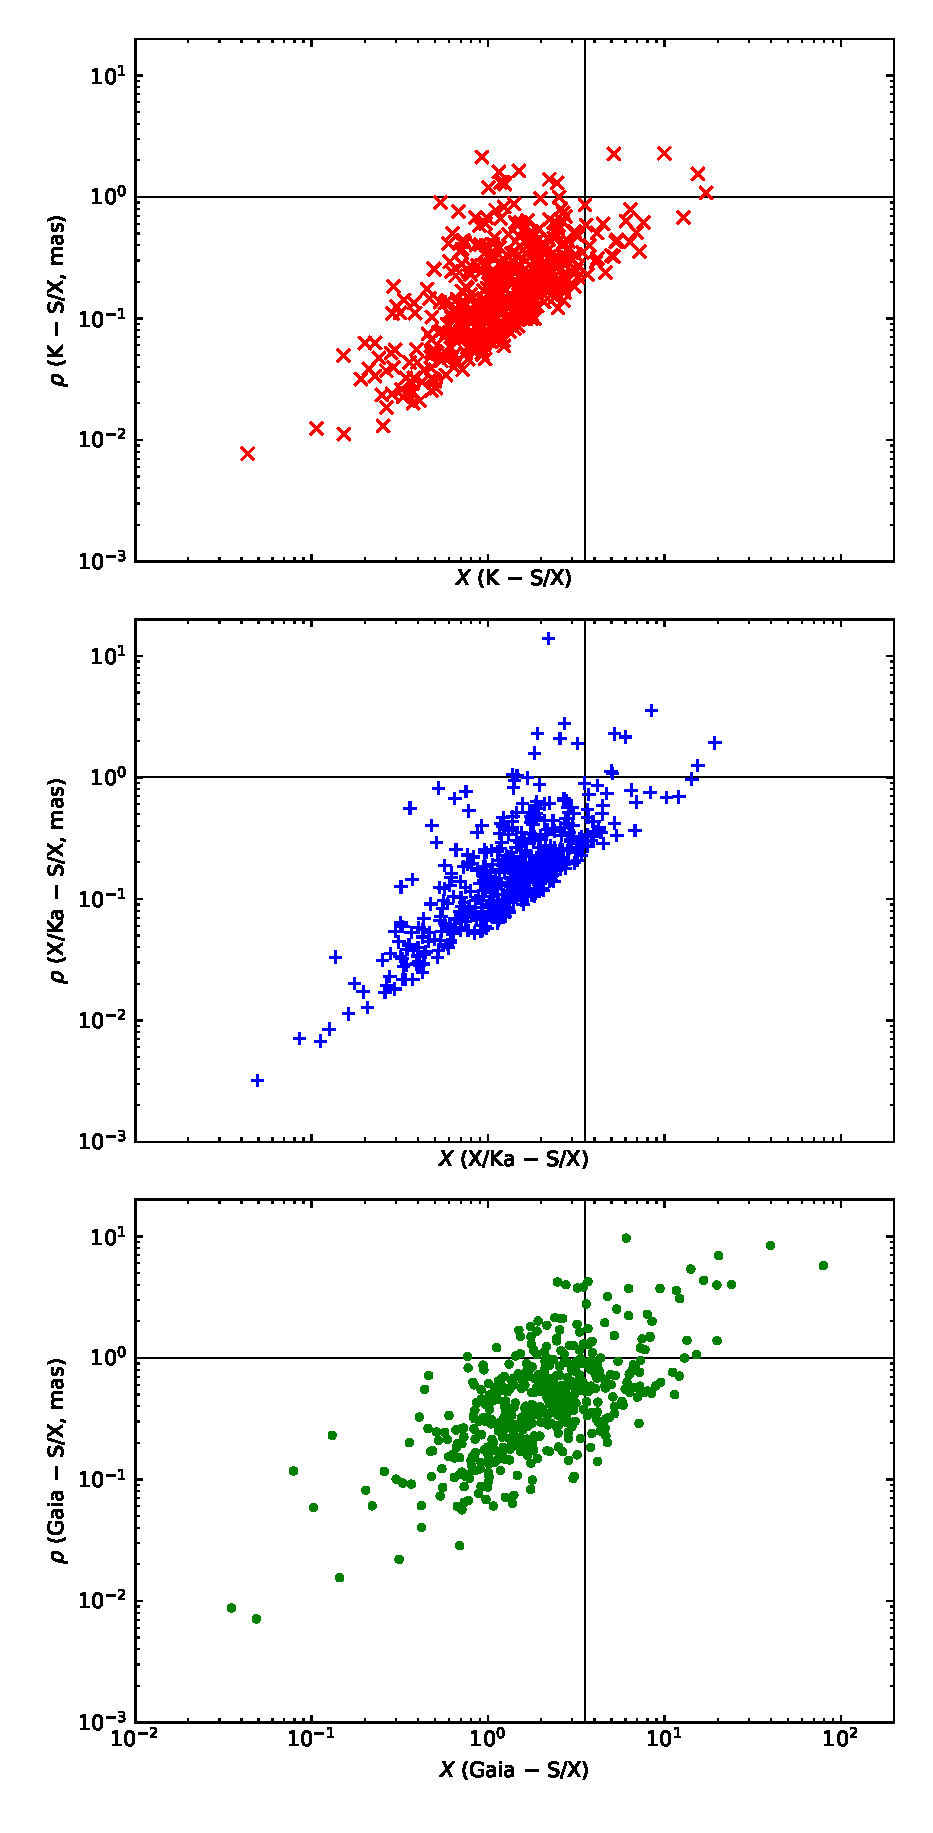
\includegraphics[width=80mm]{figs/rho-x-scatter-nosys}
    \caption[]{\label{fig:rho-x-scatter-nosys}
        Normalized position offset for common objects versus the angular separation of K, X/Ka, and Gaia with respect to S/X after aligning the frame.
        The horizontal and vertical line indicates the limit of 1\,mas and $X_0=3.52$ on the normalized separation and angular separation, respectively.
    }
\end{figure}
%===========================================================================

%% {fig:k-sx-scatter-nosys}
%===========================================================================
\begin{figure}[hbtp]
    \centering
    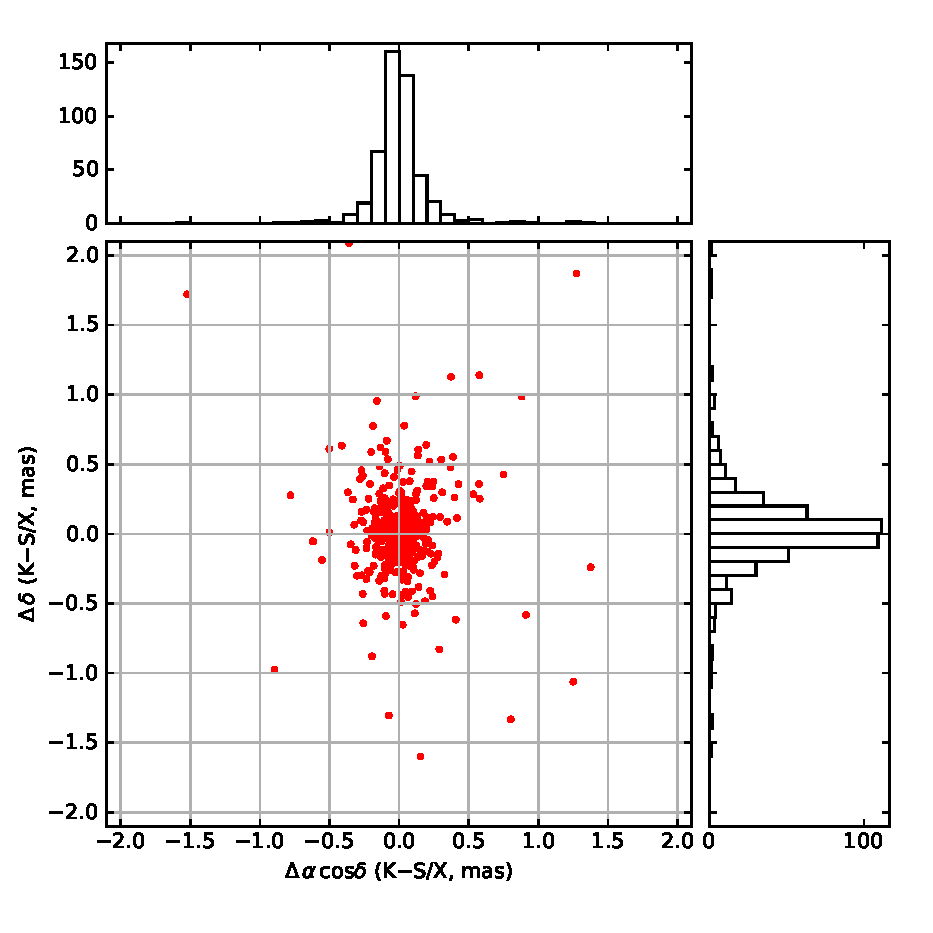
\includegraphics[width=80mm]{figs/k-sx-scatter-nosys}
    \caption[]{\label{fig:k-sx-scatter-nosys}
        Position offset scatter for common objects between S/X and K, in the sense of `K$-$S/X' after aligning the frame.
    }
\end{figure}
%===========================================================================

%% {fig:xka-sx-scatter-nosys}
%===========================================================================
\begin{figure}[hbtp]
    \centering
    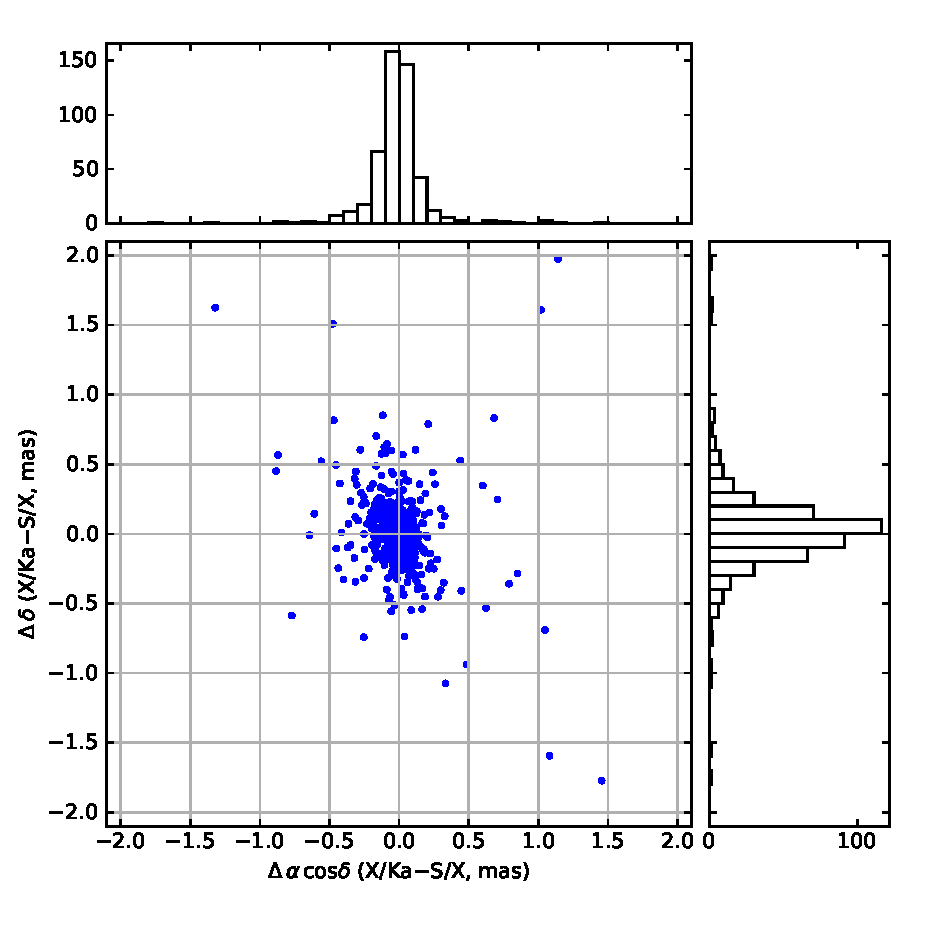
\includegraphics[width=80mm]{figs/xka-sx-scatter-nosys}
    \caption[]{\label{fig:xka-sx-scatter-nosys}
        Position offset scatter for common objects between S/X and X/Ka, in the sense of `X/Ka$-$S/X' after aligning the frame.
    }
\end{figure}
%===========================================================================

%% {fig:gdr2-sx-scatter-nosys}
%===========================================================================
\begin{figure}[hbtp]
    \centering
    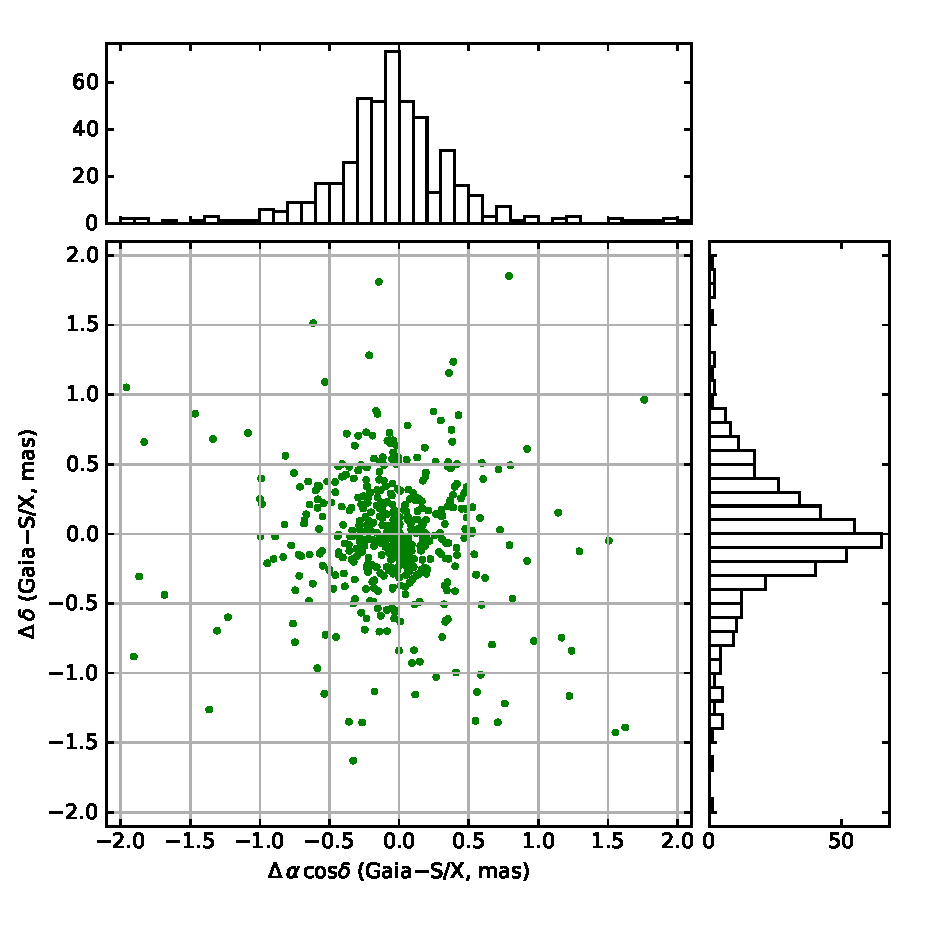
\includegraphics[width=80mm]{figs/gdr2-sx-scatter-nosys}
    \caption[]{\label{fig:gdr2-sx-scatter-nosyst}
        Position offset scatter for common objects between S/X and Gaia, in the sense of `Gaia$-$S/X' after aligning the frame.
    }
\end{figure}
%===========================================================================

%% {fig:pa-nosys}
%===========================================================================
\begin{figure}[hbtp]
    \centering
    \includegraphics[width=80mm]{figs/pa-nosys}
    \caption[]{\label{fig:pa-nosys}
        Distribution of position angle for K-band, X/Ka-band, and Gaia position as seen from S/X-band position. 
    }
\end{figure}
%===========================================================================

%% {fig:pa-nosys}
%===========================================================================
\begin{figure*}[hbtp]
    \centering
    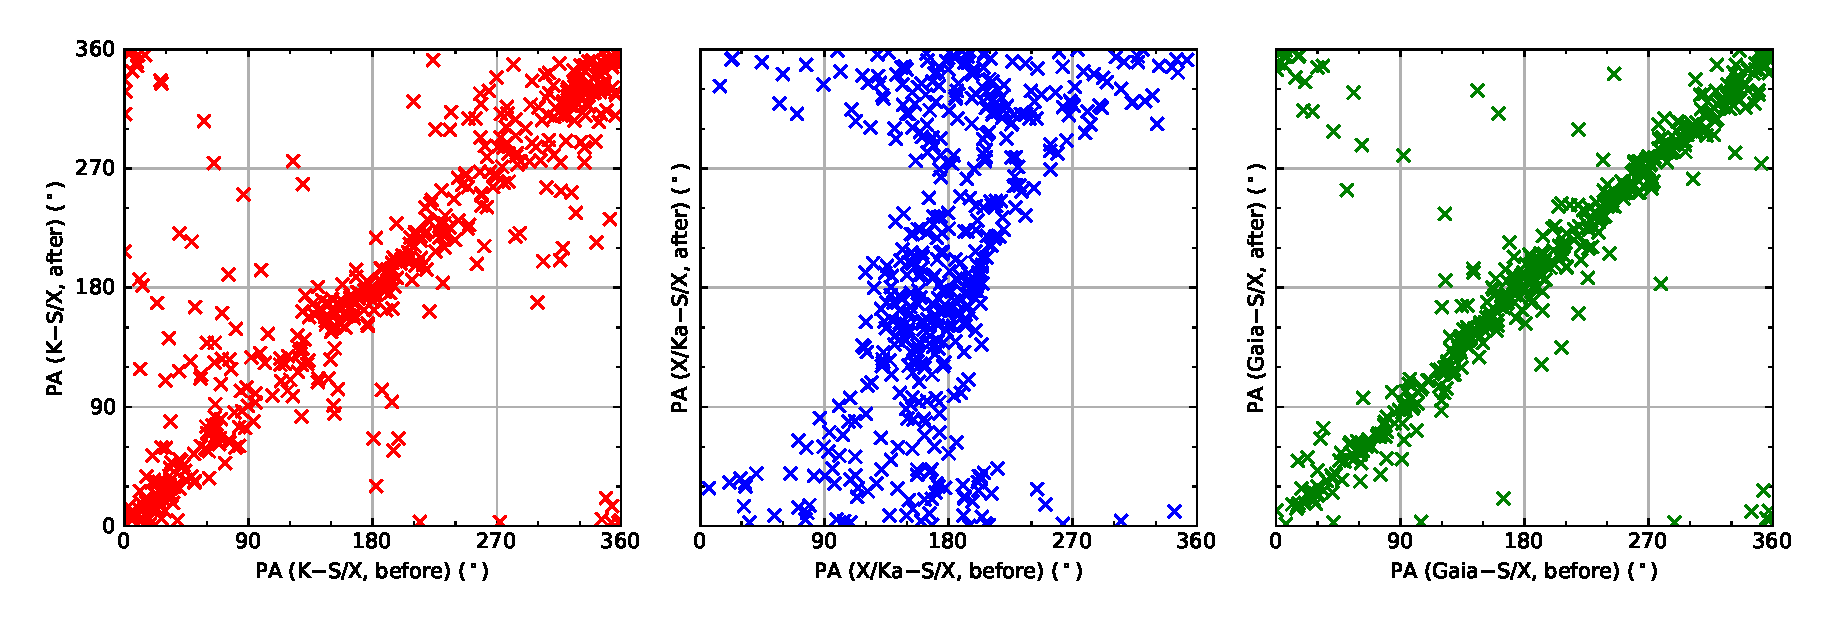
\includegraphics[width=160mm]{figs/pa-diff-from-sys}
    \caption[]{\label{fig:pa-diff-from-sys}
        Distribution of position angle before and after aligning the frames. 
    }
\end{figure*}
%===========================================================================

%% {fig:pa-diff-nosys}
%===========================================================================
\begin{figure}[hbtp]
    \centering
    \includegraphics[width=80mm]{figs/pa-diff-nosys}
    \caption[]{\label{fig:pa-diff-nosys}
        Distribution of included angle amongst K, X/Ka, and Gaia positions with respective to S/X position. 
    }
\end{figure}
%===========================================================================

%%%%%%%%%%%%%%%%%%%%%%%%%%%%%%%%%%%%%%%%%%%%%%%%%%%%%%%%%%%%%%%%%%%%%%%%%%%%
\subsection{correlation between PA and Gaia proper motion} \label{subsec:pa-pm}
%%%%%%%%%%%%%%%%%%%%%%%%%%%%%%%%%%%%%%%%%%%%%%%%%%%%%%%%%%%%%%%%%%%%%%%%%%%%

In this short section, I studied the correlation between the position offset and Gaia proper motion.
The included angle between Gaia proper motion vector and three position offset vectors were calculated and their distribution is shown in Fig.~\ref{fig:pa-pm-nosys}.
There is no clear preference in the included angles.
In this sense, the position offsets do not correlate with the proper motion measured by Gaia.

%% {fig:pa-pm-nosys}
%===========================================================================
\begin{figure}[hbtp]
    \centering
    \includegraphics[width=80mm]{figs/pa-pm-nosys}
    \caption[]{\label{fig:pa-pm-nosys}
        Distribution of included angle between K, X/Ka, and Gaia positions with respective to S/X position and Gaia DR2 proper motions. 
    }
\end{figure}
%===========================================================================


%%%%%%%%%%%%%%%%%%%%%%%%%%%%%%%%%%%%%%%%%%%%%%%%%%%%%%%%%%%%%%%%%%%%%%%%%%%%
\section{Conclusions} \label{sec:conclusions}
%%%%%%%%%%%%%%%%%%%%%%%%%%%%%%%%%%%%%%%%%%%%%%%%%%%%%%%%%%%%%%%%%%%%%%%%%%%%

I find possible clues to show that for some quasars, the K-, X/Ka-band, and Gaia positions align in the same direction (maybe it is the direction of jet) as seen from S/X position.

What to do next?\\
(1) Select quasars with similar PAs at K, X/Ka, and Gaia.
(2) Look at distribution of PA for these quasar to see if the result is biased by the declination error, that is, to see if for these objects the PA is close to $0\,^\circ$, $180\,^\circ$, and $360\,^\circ$.\\
(3) Look at their imaging to find any interesting feature.\\
(4) Find their jet directions.\\
(5) Only look at quasar with a significant position offset, e.g., $X>1$. Only for these, the PA calculation is meaningful. 

%%%%%%%%%%%%%%%%%%%%%%%%%%%%%%%%%%%%%%%%%%%%%%%%%%%%%%%%%%%%%%%%%%%%%%%%%%%%
\begin{acknowledgements}
  We are much indebted to Rob Rutten for exemplary instruction.
  We made much use of NASA's Astrophysics Data System.
\end{acknowledgements}


%%%%%%%%%%%%%%%%%%%%%%%%%%%%%%%%%%%%%%%%%%%%%%%%%%%%%%%%%%%%%%%%%%%%%%%%%%%%
%% references
%\bibliographystyle{aa-note} %% aa.bst but adding links and notes to references
%%\raggedright              %% only for adsaa with dvips, not for pdflatex
%\bibliography{XXX}          %% XXX.bib = your Bibtex entries copied from ADS

\end{document}

